\mbox{$\displaystyle -\,$\,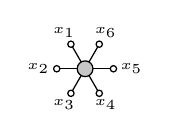
\begin{tikzpicture}[x=0.500cm, y=0.500cm, line width=0.450pt, baseline={([yshift=-0.6ex]0,0)}]
  \draw (-0.360,0.624) -- (0.000,0.000);
  \draw (-0.720,0.000) -- (0.000,0.000);
  \draw (-0.360,-0.624) -- (0.000,0.000);
  \draw (0.360,-0.624) -- (0.000,0.000);
  \draw (0.720,0.000) -- (0.000,0.000);
  \draw (0.360,0.624) -- (0.000,0.000);
  \draw[fill=black!22] (0.000,0.000) circle (0.200);
  \draw[fill=white] (-0.360,0.624) circle (0.080);
  \draw[fill=white] (-0.720,0.000) circle (0.080);
  \draw[fill=white] (-0.360,-0.624) circle (0.080);
  \draw[fill=white] (0.360,-0.624) circle (0.080);
  \draw[fill=white] (0.720,0.000) circle (0.080);
  \draw[fill=white] (0.360,0.624) circle (0.080);
  \node[font=\tiny, inner sep=0pt, anchor=300] at (-0.445,0.771) {$x_{1}$};
  \node[font=\tiny, inner sep=0pt, anchor=0] at (-0.890,0.000) {$x_{2}$};
  \node[font=\tiny, inner sep=0pt, anchor=60] at (-0.445,-0.771) {$x_{3}$};
  \node[font=\tiny, inner sep=0pt, anchor=120] at (0.445,-0.771) {$x_{4}$};
  \node[font=\tiny, inner sep=0pt, anchor=180] at (0.890,0.000) {$x_{5}$};
  \node[font=\tiny, inner sep=0pt, anchor=240] at (0.445,0.771) {$x_{6}$};
\end{tikzpicture}}
\diagramgap
\mbox{$\displaystyle +\,$\,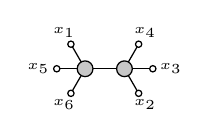
\begin{tikzpicture}[x=0.500cm, y=0.500cm, line width=0.450pt, baseline={([yshift=-0.6ex]0,0)}]
  \draw (-0.860,0.624) -- (-0.500,0.000);
  \draw (0.860,-0.624) -- (0.500,0.000);
  \draw (1.220,0.000) -- (0.500,0.000);
  \draw (0.860,0.624) -- (0.500,0.000);
  \draw (-1.220,0.000) -- (-0.500,0.000);
  \draw (-0.860,-0.624) -- (-0.500,0.000);
  \draw (-0.500,0.000) -- (0.500,0.000);
  \draw[fill=black!22] (-0.500,0.000) circle (0.200);
  \draw[fill=black!22] (0.500,0.000) circle (0.200);
  \draw[fill=white] (-0.860,0.624) circle (0.080);
  \draw[fill=white] (0.860,-0.624) circle (0.080);
  \draw[fill=white] (1.220,0.000) circle (0.080);
  \draw[fill=white] (0.860,0.624) circle (0.080);
  \draw[fill=white] (-1.220,0.000) circle (0.080);
  \draw[fill=white] (-0.860,-0.624) circle (0.080);
  \node[font=\tiny, inner sep=0pt, anchor=300] at (-0.945,0.771) {$x_{1}$};
  \node[font=\tiny, inner sep=0pt, anchor=120] at (0.945,-0.771) {$x_{2}$};
  \node[font=\tiny, inner sep=0pt, anchor=180] at (1.390,0.000) {$x_{3}$};
  \node[font=\tiny, inner sep=0pt, anchor=240] at (0.945,0.771) {$x_{4}$};
  \node[font=\tiny, inner sep=0pt, anchor=0] at (-1.390,0.000) {$x_{5}$};
  \node[font=\tiny, inner sep=0pt, anchor=60] at (-0.945,-0.771) {$x_{6}$};
\end{tikzpicture}}
\diagramgap
\mbox{$\displaystyle -\,$\,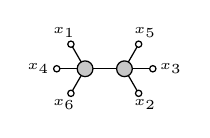
\begin{tikzpicture}[x=0.500cm, y=0.500cm, line width=0.450pt, baseline={([yshift=-0.6ex]0,0)}]
  \draw (-0.860,0.624) -- (-0.500,0.000);
  \draw (0.860,-0.624) -- (0.500,0.000);
  \draw (1.220,0.000) -- (0.500,0.000);
  \draw (-1.220,0.000) -- (-0.500,0.000);
  \draw (0.860,0.624) -- (0.500,0.000);
  \draw (-0.860,-0.624) -- (-0.500,0.000);
  \draw (-0.500,0.000) -- (0.500,0.000);
  \draw[fill=black!22] (-0.500,0.000) circle (0.200);
  \draw[fill=black!22] (0.500,0.000) circle (0.200);
  \draw[fill=white] (-0.860,0.624) circle (0.080);
  \draw[fill=white] (0.860,-0.624) circle (0.080);
  \draw[fill=white] (1.220,0.000) circle (0.080);
  \draw[fill=white] (-1.220,0.000) circle (0.080);
  \draw[fill=white] (0.860,0.624) circle (0.080);
  \draw[fill=white] (-0.860,-0.624) circle (0.080);
  \node[font=\tiny, inner sep=0pt, anchor=300] at (-0.945,0.771) {$x_{1}$};
  \node[font=\tiny, inner sep=0pt, anchor=120] at (0.945,-0.771) {$x_{2}$};
  \node[font=\tiny, inner sep=0pt, anchor=180] at (1.390,0.000) {$x_{3}$};
  \node[font=\tiny, inner sep=0pt, anchor=0] at (-1.390,0.000) {$x_{4}$};
  \node[font=\tiny, inner sep=0pt, anchor=240] at (0.945,0.771) {$x_{5}$};
  \node[font=\tiny, inner sep=0pt, anchor=60] at (-0.945,-0.771) {$x_{6}$};
\end{tikzpicture}}
\diagramgap
\mbox{$\displaystyle +\,$\,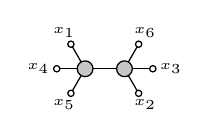
\begin{tikzpicture}[x=0.500cm, y=0.500cm, line width=0.450pt, baseline={([yshift=-0.6ex]0,0)}]
  \draw (-0.860,0.624) -- (-0.500,0.000);
  \draw (0.860,-0.624) -- (0.500,0.000);
  \draw (1.220,0.000) -- (0.500,0.000);
  \draw (-1.220,0.000) -- (-0.500,0.000);
  \draw (-0.860,-0.624) -- (-0.500,0.000);
  \draw (0.860,0.624) -- (0.500,0.000);
  \draw (-0.500,0.000) -- (0.500,0.000);
  \draw[fill=black!22] (-0.500,0.000) circle (0.200);
  \draw[fill=black!22] (0.500,0.000) circle (0.200);
  \draw[fill=white] (-0.860,0.624) circle (0.080);
  \draw[fill=white] (0.860,-0.624) circle (0.080);
  \draw[fill=white] (1.220,0.000) circle (0.080);
  \draw[fill=white] (-1.220,0.000) circle (0.080);
  \draw[fill=white] (-0.860,-0.624) circle (0.080);
  \draw[fill=white] (0.860,0.624) circle (0.080);
  \node[font=\tiny, inner sep=0pt, anchor=300] at (-0.945,0.771) {$x_{1}$};
  \node[font=\tiny, inner sep=0pt, anchor=120] at (0.945,-0.771) {$x_{2}$};
  \node[font=\tiny, inner sep=0pt, anchor=180] at (1.390,0.000) {$x_{3}$};
  \node[font=\tiny, inner sep=0pt, anchor=0] at (-1.390,0.000) {$x_{4}$};
  \node[font=\tiny, inner sep=0pt, anchor=60] at (-0.945,-0.771) {$x_{5}$};
  \node[font=\tiny, inner sep=0pt, anchor=240] at (0.945,0.771) {$x_{6}$};
\end{tikzpicture}}
\diagramgap
\mbox{$\displaystyle +\,$\,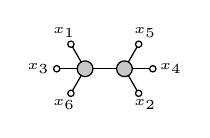
\begin{tikzpicture}[x=0.500cm, y=0.500cm, line width=0.450pt, baseline={([yshift=-0.6ex]0,0)}]
  \draw (-0.860,0.624) -- (-0.500,0.000);
  \draw (0.860,-0.624) -- (0.500,0.000);
  \draw (-1.220,0.000) -- (-0.500,0.000);
  \draw (1.220,0.000) -- (0.500,0.000);
  \draw (0.860,0.624) -- (0.500,0.000);
  \draw (-0.860,-0.624) -- (-0.500,0.000);
  \draw (-0.500,0.000) -- (0.500,0.000);
  \draw[fill=black!22] (-0.500,0.000) circle (0.200);
  \draw[fill=black!22] (0.500,0.000) circle (0.200);
  \draw[fill=white] (-0.860,0.624) circle (0.080);
  \draw[fill=white] (0.860,-0.624) circle (0.080);
  \draw[fill=white] (-1.220,0.000) circle (0.080);
  \draw[fill=white] (1.220,0.000) circle (0.080);
  \draw[fill=white] (0.860,0.624) circle (0.080);
  \draw[fill=white] (-0.860,-0.624) circle (0.080);
  \node[font=\tiny, inner sep=0pt, anchor=300] at (-0.945,0.771) {$x_{1}$};
  \node[font=\tiny, inner sep=0pt, anchor=120] at (0.945,-0.771) {$x_{2}$};
  \node[font=\tiny, inner sep=0pt, anchor=0] at (-1.390,0.000) {$x_{3}$};
  \node[font=\tiny, inner sep=0pt, anchor=180] at (1.390,0.000) {$x_{4}$};
  \node[font=\tiny, inner sep=0pt, anchor=240] at (0.945,0.771) {$x_{5}$};
  \node[font=\tiny, inner sep=0pt, anchor=60] at (-0.945,-0.771) {$x_{6}$};
\end{tikzpicture}}
\diagramgap
\mbox{$\displaystyle -\,$\,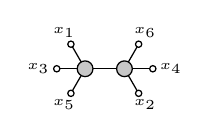
\begin{tikzpicture}[x=0.500cm, y=0.500cm, line width=0.450pt, baseline={([yshift=-0.6ex]0,0)}]
  \draw (-0.860,0.624) -- (-0.500,0.000);
  \draw (0.860,-0.624) -- (0.500,0.000);
  \draw (-1.220,0.000) -- (-0.500,0.000);
  \draw (1.220,0.000) -- (0.500,0.000);
  \draw (-0.860,-0.624) -- (-0.500,0.000);
  \draw (0.860,0.624) -- (0.500,0.000);
  \draw (-0.500,0.000) -- (0.500,0.000);
  \draw[fill=black!22] (-0.500,0.000) circle (0.200);
  \draw[fill=black!22] (0.500,0.000) circle (0.200);
  \draw[fill=white] (-0.860,0.624) circle (0.080);
  \draw[fill=white] (0.860,-0.624) circle (0.080);
  \draw[fill=white] (-1.220,0.000) circle (0.080);
  \draw[fill=white] (1.220,0.000) circle (0.080);
  \draw[fill=white] (-0.860,-0.624) circle (0.080);
  \draw[fill=white] (0.860,0.624) circle (0.080);
  \node[font=\tiny, inner sep=0pt, anchor=300] at (-0.945,0.771) {$x_{1}$};
  \node[font=\tiny, inner sep=0pt, anchor=120] at (0.945,-0.771) {$x_{2}$};
  \node[font=\tiny, inner sep=0pt, anchor=0] at (-1.390,0.000) {$x_{3}$};
  \node[font=\tiny, inner sep=0pt, anchor=180] at (1.390,0.000) {$x_{4}$};
  \node[font=\tiny, inner sep=0pt, anchor=60] at (-0.945,-0.771) {$x_{5}$};
  \node[font=\tiny, inner sep=0pt, anchor=240] at (0.945,0.771) {$x_{6}$};
\end{tikzpicture}}
\diagramgap
\mbox{$\displaystyle +\,$\,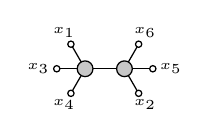
\begin{tikzpicture}[x=0.500cm, y=0.500cm, line width=0.450pt, baseline={([yshift=-0.6ex]0,0)}]
  \draw (-0.860,0.624) -- (-0.500,0.000);
  \draw (0.860,-0.624) -- (0.500,0.000);
  \draw (-1.220,0.000) -- (-0.500,0.000);
  \draw (-0.860,-0.624) -- (-0.500,0.000);
  \draw (1.220,0.000) -- (0.500,0.000);
  \draw (0.860,0.624) -- (0.500,0.000);
  \draw (-0.500,0.000) -- (0.500,0.000);
  \draw[fill=black!22] (-0.500,0.000) circle (0.200);
  \draw[fill=black!22] (0.500,0.000) circle (0.200);
  \draw[fill=white] (-0.860,0.624) circle (0.080);
  \draw[fill=white] (0.860,-0.624) circle (0.080);
  \draw[fill=white] (-1.220,0.000) circle (0.080);
  \draw[fill=white] (-0.860,-0.624) circle (0.080);
  \draw[fill=white] (1.220,0.000) circle (0.080);
  \draw[fill=white] (0.860,0.624) circle (0.080);
  \node[font=\tiny, inner sep=0pt, anchor=300] at (-0.945,0.771) {$x_{1}$};
  \node[font=\tiny, inner sep=0pt, anchor=120] at (0.945,-0.771) {$x_{2}$};
  \node[font=\tiny, inner sep=0pt, anchor=0] at (-1.390,0.000) {$x_{3}$};
  \node[font=\tiny, inner sep=0pt, anchor=60] at (-0.945,-0.771) {$x_{4}$};
  \node[font=\tiny, inner sep=0pt, anchor=180] at (1.390,0.000) {$x_{5}$};
  \node[font=\tiny, inner sep=0pt, anchor=240] at (0.945,0.771) {$x_{6}$};
\end{tikzpicture}}
\diagramgap
\mbox{$\displaystyle -\,$\,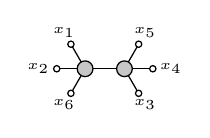
\begin{tikzpicture}[x=0.500cm, y=0.500cm, line width=0.450pt, baseline={([yshift=-0.6ex]0,0)}]
  \draw (-0.860,0.624) -- (-0.500,0.000);
  \draw (-1.220,0.000) -- (-0.500,0.000);
  \draw (0.860,-0.624) -- (0.500,0.000);
  \draw (1.220,0.000) -- (0.500,0.000);
  \draw (0.860,0.624) -- (0.500,0.000);
  \draw (-0.860,-0.624) -- (-0.500,0.000);
  \draw (-0.500,0.000) -- (0.500,0.000);
  \draw[fill=black!22] (-0.500,0.000) circle (0.200);
  \draw[fill=black!22] (0.500,0.000) circle (0.200);
  \draw[fill=white] (-0.860,0.624) circle (0.080);
  \draw[fill=white] (-1.220,0.000) circle (0.080);
  \draw[fill=white] (0.860,-0.624) circle (0.080);
  \draw[fill=white] (1.220,0.000) circle (0.080);
  \draw[fill=white] (0.860,0.624) circle (0.080);
  \draw[fill=white] (-0.860,-0.624) circle (0.080);
  \node[font=\tiny, inner sep=0pt, anchor=300] at (-0.945,0.771) {$x_{1}$};
  \node[font=\tiny, inner sep=0pt, anchor=0] at (-1.390,0.000) {$x_{2}$};
  \node[font=\tiny, inner sep=0pt, anchor=120] at (0.945,-0.771) {$x_{3}$};
  \node[font=\tiny, inner sep=0pt, anchor=180] at (1.390,0.000) {$x_{4}$};
  \node[font=\tiny, inner sep=0pt, anchor=240] at (0.945,0.771) {$x_{5}$};
  \node[font=\tiny, inner sep=0pt, anchor=60] at (-0.945,-0.771) {$x_{6}$};
\end{tikzpicture}}
\diagramgap
\mbox{$\displaystyle +\,$\,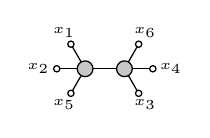
\begin{tikzpicture}[x=0.500cm, y=0.500cm, line width=0.450pt, baseline={([yshift=-0.6ex]0,0)}]
  \draw (-0.860,0.624) -- (-0.500,0.000);
  \draw (-1.220,0.000) -- (-0.500,0.000);
  \draw (0.860,-0.624) -- (0.500,0.000);
  \draw (1.220,0.000) -- (0.500,0.000);
  \draw (-0.860,-0.624) -- (-0.500,0.000);
  \draw (0.860,0.624) -- (0.500,0.000);
  \draw (-0.500,0.000) -- (0.500,0.000);
  \draw[fill=black!22] (-0.500,0.000) circle (0.200);
  \draw[fill=black!22] (0.500,0.000) circle (0.200);
  \draw[fill=white] (-0.860,0.624) circle (0.080);
  \draw[fill=white] (-1.220,0.000) circle (0.080);
  \draw[fill=white] (0.860,-0.624) circle (0.080);
  \draw[fill=white] (1.220,0.000) circle (0.080);
  \draw[fill=white] (-0.860,-0.624) circle (0.080);
  \draw[fill=white] (0.860,0.624) circle (0.080);
  \node[font=\tiny, inner sep=0pt, anchor=300] at (-0.945,0.771) {$x_{1}$};
  \node[font=\tiny, inner sep=0pt, anchor=0] at (-1.390,0.000) {$x_{2}$};
  \node[font=\tiny, inner sep=0pt, anchor=120] at (0.945,-0.771) {$x_{3}$};
  \node[font=\tiny, inner sep=0pt, anchor=180] at (1.390,0.000) {$x_{4}$};
  \node[font=\tiny, inner sep=0pt, anchor=60] at (-0.945,-0.771) {$x_{5}$};
  \node[font=\tiny, inner sep=0pt, anchor=240] at (0.945,0.771) {$x_{6}$};
\end{tikzpicture}}
\diagramgap
\mbox{$\displaystyle -\,$\,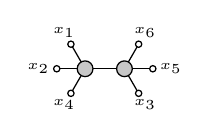
\begin{tikzpicture}[x=0.500cm, y=0.500cm, line width=0.450pt, baseline={([yshift=-0.6ex]0,0)}]
  \draw (-0.860,0.624) -- (-0.500,0.000);
  \draw (-1.220,0.000) -- (-0.500,0.000);
  \draw (0.860,-0.624) -- (0.500,0.000);
  \draw (-0.860,-0.624) -- (-0.500,0.000);
  \draw (1.220,0.000) -- (0.500,0.000);
  \draw (0.860,0.624) -- (0.500,0.000);
  \draw (-0.500,0.000) -- (0.500,0.000);
  \draw[fill=black!22] (-0.500,0.000) circle (0.200);
  \draw[fill=black!22] (0.500,0.000) circle (0.200);
  \draw[fill=white] (-0.860,0.624) circle (0.080);
  \draw[fill=white] (-1.220,0.000) circle (0.080);
  \draw[fill=white] (0.860,-0.624) circle (0.080);
  \draw[fill=white] (-0.860,-0.624) circle (0.080);
  \draw[fill=white] (1.220,0.000) circle (0.080);
  \draw[fill=white] (0.860,0.624) circle (0.080);
  \node[font=\tiny, inner sep=0pt, anchor=300] at (-0.945,0.771) {$x_{1}$};
  \node[font=\tiny, inner sep=0pt, anchor=0] at (-1.390,0.000) {$x_{2}$};
  \node[font=\tiny, inner sep=0pt, anchor=120] at (0.945,-0.771) {$x_{3}$};
  \node[font=\tiny, inner sep=0pt, anchor=60] at (-0.945,-0.771) {$x_{4}$};
  \node[font=\tiny, inner sep=0pt, anchor=180] at (1.390,0.000) {$x_{5}$};
  \node[font=\tiny, inner sep=0pt, anchor=240] at (0.945,0.771) {$x_{6}$};
\end{tikzpicture}}
\diagramgap
\mbox{$\displaystyle +\,$\,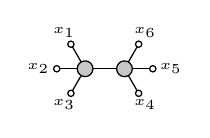
\begin{tikzpicture}[x=0.500cm, y=0.500cm, line width=0.450pt, baseline={([yshift=-0.6ex]0,0)}]
  \draw (-0.860,0.624) -- (-0.500,0.000);
  \draw (-1.220,0.000) -- (-0.500,0.000);
  \draw (-0.860,-0.624) -- (-0.500,0.000);
  \draw (0.860,-0.624) -- (0.500,0.000);
  \draw (1.220,0.000) -- (0.500,0.000);
  \draw (0.860,0.624) -- (0.500,0.000);
  \draw (-0.500,0.000) -- (0.500,0.000);
  \draw[fill=black!22] (-0.500,0.000) circle (0.200);
  \draw[fill=black!22] (0.500,0.000) circle (0.200);
  \draw[fill=white] (-0.860,0.624) circle (0.080);
  \draw[fill=white] (-1.220,0.000) circle (0.080);
  \draw[fill=white] (-0.860,-0.624) circle (0.080);
  \draw[fill=white] (0.860,-0.624) circle (0.080);
  \draw[fill=white] (1.220,0.000) circle (0.080);
  \draw[fill=white] (0.860,0.624) circle (0.080);
  \node[font=\tiny, inner sep=0pt, anchor=300] at (-0.945,0.771) {$x_{1}$};
  \node[font=\tiny, inner sep=0pt, anchor=0] at (-1.390,0.000) {$x_{2}$};
  \node[font=\tiny, inner sep=0pt, anchor=60] at (-0.945,-0.771) {$x_{3}$};
  \node[font=\tiny, inner sep=0pt, anchor=120] at (0.945,-0.771) {$x_{4}$};
  \node[font=\tiny, inner sep=0pt, anchor=180] at (1.390,0.000) {$x_{5}$};
  \node[font=\tiny, inner sep=0pt, anchor=240] at (0.945,0.771) {$x_{6}$};
\end{tikzpicture}}
